\documentclass{standalone}

\usepackage{tikz}
\usetikzlibrary{arrows.meta}


\begin{document}

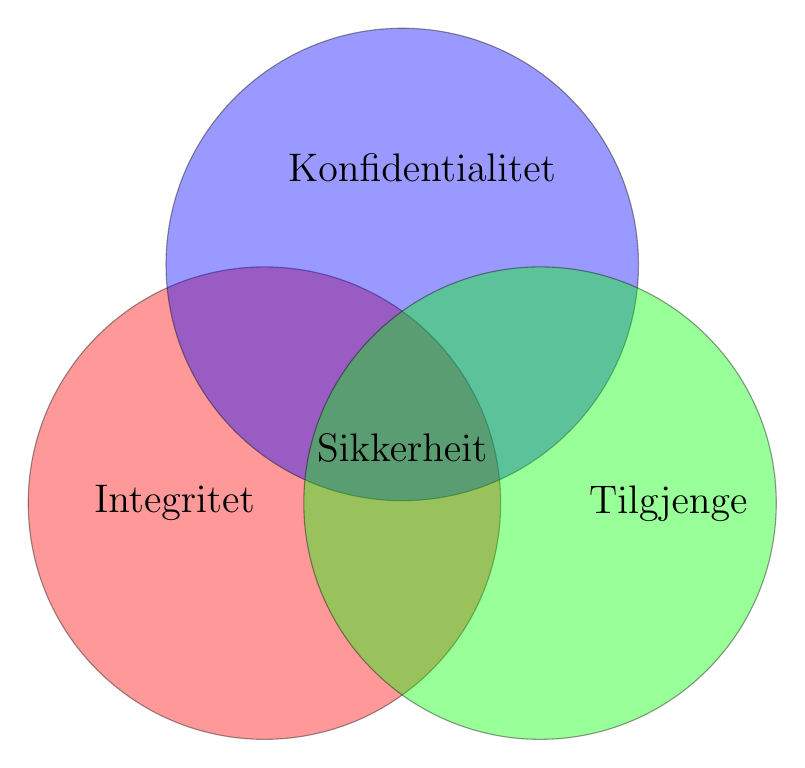
\begin{tikzpicture}
  \tikzset{venn circle/.style={draw,circle,minimum width=6cm,fill=#1,opacity=0.4}}

  \node [venn circle = red] (A) at (0,0) {};
  \node [venn circle = blue] (B) at (60:35mm) {};
  \node [venn circle = green] (C) at (0:35mm) {};

   \node [left] at (0,0) {\Large Integritet};
   \node [above] [yshift=5mm] at (60:4cm) {{\Large Konfidentialitet}};
   \node [right] at (0:40mm) {\Large Tilgjenge};

  % \node[left] at (barycentric cs:A=1/2,B=1/2 ) {};
  % \node[below] at (barycentric cs:A=1/2,C=1/2 ) {};
  % \node[right] at (barycentric cs:B=1/2,C=1/2 ) {};
  \node[below] at (barycentric cs:A=1/3,B=1/3,C=1/3 ){\Large Sikkerheit};
\end{tikzpicture}

\end{document}
